%!TEX root = ../main.tex
%%%%%%%%%%%%%%%%%%%%%%%%%%%%%%%%%%
% Links:
%
% Difficulty:
% Companies: 
%%%%%%%%%%%%%%%%%%%%%%%%%%%%%%%%%%


\chapter{Least Recently Used Cache}
\label{ch:LRU_cache}
\section*{Introduction}
Caches are piece of hardwoare of software systems responsible to store data that allow the system to respond to future requests faster. Usually such data is the result of earlier computation 
of it could data that was copied over from somewhere else  (following the principle of temporal and spatial locality which states that applications are more likely to access data that has been accessed recently and/or that sit close in memory).  
Caches are essential piece of nowadays computer systems and we find them at every level: from CPUs and HDDs (see Figure \ref{fig:LRU_cache:cpu_cache}) that have dedicated expensive blocks of memory that for temporary storage of data that is likely to be used again, to 
browsers or webserver (see Figure \ref{fig:LRU_cache:web_cache}) that use caches to try and lower the latency of your browsing.


Clearly caches have finite size and eventually they get full and therefore we run into the issue of deciding what to delete from it in order to make some space available for the new data. There are many policies that can be employed here like for example:
\begin{itemize}
	\item LRU: discards the least recently used items first;
	\item FIFO: evice the oldest data first (regardless of whether it has been accessed recently);
	\item RR: (random replacement) that, as the name suggests, removes one or more random cache entries.
\end{itemize}

The problem we will solve in this chapter is about implementing a LRU cache so that all of its supported operation are carried out with the best time efficiency possible. As we will see, solving this problem by making all operations $log(n)$ is actually pretty easy, but 


\begin{figure}
	\centering
	\begin{subfigure}[t]{0.49\textwidth}
		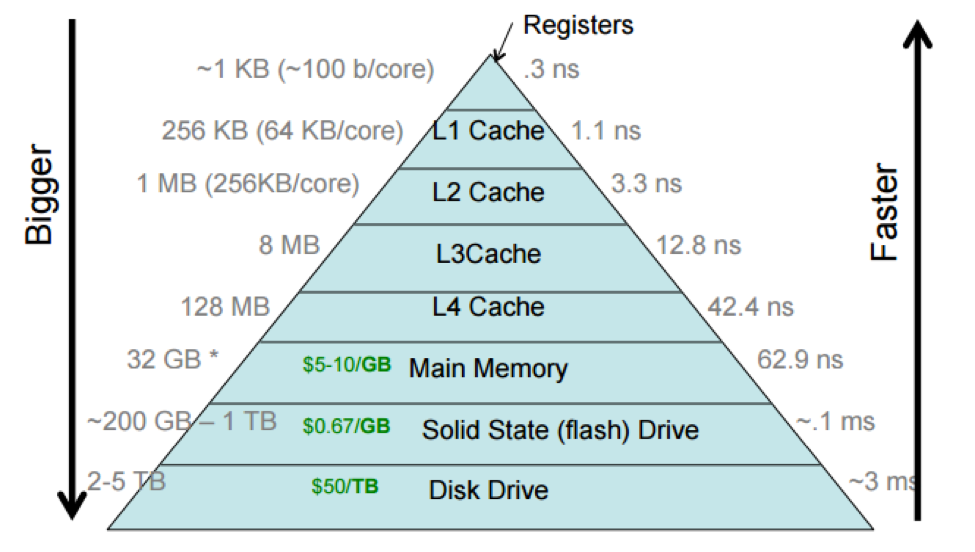
\includegraphics[width=1\linewidth]{sources/LRU_cache/images/cpu_caches}
		\caption{Caches (notice that there are multiple level of it) are at the top of the memory hierarchy of modern computers. See Table \ref{tab:refernce_latencies} for a more detailed account of the latencies figures for each and every memory level of the hierarchy. The figures on size and latency showed are for a typical desktop computer. Use \inline{getconf -a | grep CACHE} or \inline{lscpu} to check the actual cache size in your system.}
		\label{fig:LRU_cache:cpu_cache}
	 \end{subfigure}
	\hfill
	\begin{subfigure}[t]{0.49\textwidth}
		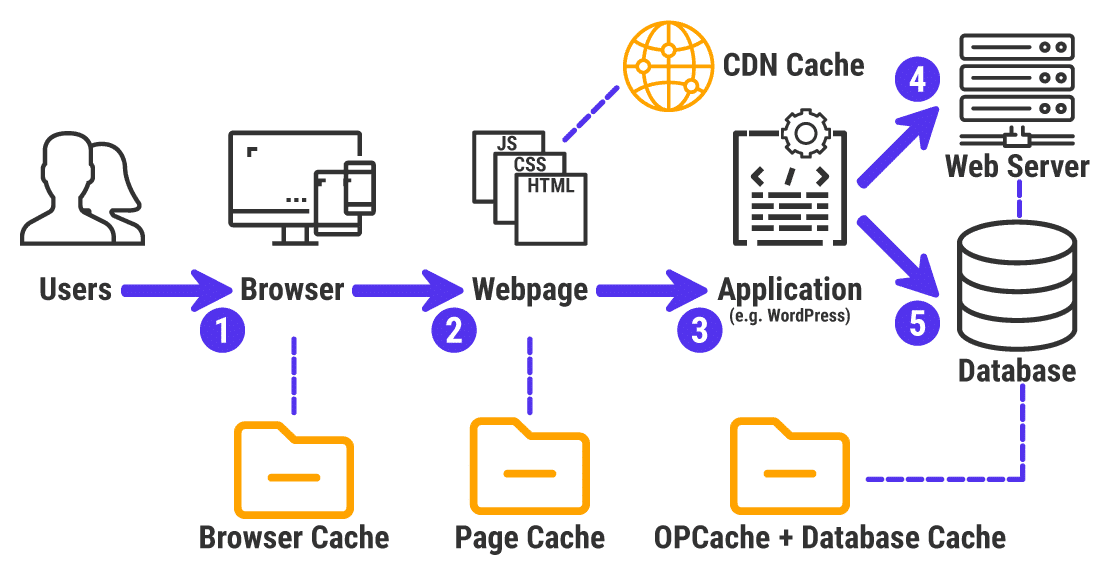
\includegraphics[width=1\linewidth]{sources/LRU_cache/images/web_caches}
		\caption{Caches in the internet. We can see caches being used at every level. Even the database might cache recently used data in memory.}
		\label{fig:LRU_cache:web_cache}
	 \end{subfigure}
	 \caption[]{}
	  \label{fig:LRU_cache:caches_example}
\end{figure}


\section{Problem statement}
\begin{exercise}
\label{example:LRU_cache:exercice1}
Implement the two two public methods of the \inline{LRUCache} interface below. The class should behave like a LRU cache of capacity \inline{n} that is given as a parameter.
\begin{itemize}
	\item \inline{std::optional<Value> get(Key k)} retuns the value associated with the key \inline{k}. If \inline{k} is not in the cache, the function returns \inline{std::nullptop}. 
	\item \inline{void put(Key k, Value v)} adds or update (depending on whether $k$ is already present in the cache or not) the pair $(k,v)$. If the cache if full i.e. has size $n$ the function evices the least recently used items before inserting $(k,v)$.
\end{itemize}

	%example1
	\begin{example}
		\label{example:LRU_cache:example1}
		\hfill \\ 
		For instance, given a cache \inline{C} of size $2$ (with char keys and int values), Table \ref{tab:LRU_cache:example1} shows the content after performing a number of operations on it.		
	\end{example}


\end{exercise}

% Please add the following required packages to your document preamble:
% \usepackage{graphicx}
\begin{table}[]
	\centering
	\resizebox{\textwidth}{!}{%
	\begin{tabular}{lllr}
		\hline
		\rowcolor[HTML]{C0C0C0} 
		\multicolumn{1}{c}{\cellcolor[HTML]{C0C0C0}\textbf{Operation}} & \multicolumn{1}{c}{\cellcolor[HTML]{C0C0C0}\textbf{Cache}} & \multicolumn{1}{c}{\cellcolor[HTML]{C0C0C0}\textbf{Return}} & \textbf{Comment} \\ \hline
	\inline{get('a')}                       & \inline{\{\}}     & \inline{std::nullopt} & \inline{'a'} $\notin C$ \\
	\inline{put('a',1)}                       & \inline{\{a=1\}}     & - & Put OK \\
	\inline{put('b',2)}                       & \inline{\{a=1\},\{b=2\}}     & - & Put OK \\
	\inline{get('a')}                       & \inline{\{a=1\},\{b=2\}}     & \inline{1} & \inline{'b'} is LRU element now \\
	\inline{get('b')}                       & \inline{\{a=1\},\{b=2\}}     & \inline{2} & \inline{'a'} is LRU element now\\
	\inline{put('c',3)}                       & \inline{\{a=1\},\{c=3\}}     & - & Put OK. \inline{'a'} evicted\\
	\inline{get('a')}                       & \inline{\{a=1\},\{c=3\}}     & \inline{std::nullopt} & \inline{'a'} $\notin C$ anymore\\
	\inline{get('b')}                       & \inline{\{a=1\},\{c=3\}}     & \inline{2} & Get OK\\
	\inline{get('c')}                       & \inline{\{a=1\},\{c=3\}}     & \inline{3} & Get OK

	\end{tabular}%
	}
	\caption{Example of behavior of the a LRU cache.}
	\label{tab:LRU_cache:example1}
	\end{table}

\section{Clarification Questions}

\begin{QandA}
	\item Is one of the two operations going to be performed more than the other?
	\begin{answered}
		\textit{No no assumpitons like this can be made. }
	\end{answered}
	
\end{QandA}

%\section{Discussion}
%\label{LRU_cache:sec:discussion}

\subsection{Brute-force}
\label{LRU_cache:sec:bruteforce}
A very basic solution can be obtained by just storing the key-value pairs alongside a integer value that marks their last usage time into a vector. If we make such vector is always sorted, then 
the \inline{get} operation can be implemented as a linear search and the \inline{put} would consist of a potential \inline{pop_back()} (that we only do when the cache is full and removes the oldest entry) followed by a \inline{push_back} 
and a sort. 
This is quite inefficient as, the \inline{get} operation would run in $O(n)$ time while the \inline{pu}t is even more expensive with its $O(n log(n))$ time complexity.

In order to improve things what we can do is to store the key-value-timestamp tuple into an \inline{std::unordered_map} and keep a vector of pairs \inline{std::vector<std::pair<Timestamp, Key>>} sorted by the first element of the pair.
Each pair in the vector contains the information about the last time a given key has been used.
If we keep this array sorted by such timestamp then we have a way of keeping track which element needs to be deleted when the cache is full.
Moreover, by storing the tuple in a hashmap we are now able to serve the \inline{get} operation in $O(1)$. The \inline{put} is still pretty expensive as it is still $O(n log(n))$ (actually if we use insertion sort this would most likely be $O(n)$ as we always insert in a almost sorted collection).

The reason why the \inline{put} is expensive is because every time we add a new element we need to sort the entire array again.
However if instead of a \inline{vector} we use a \inline{map} then we can continue to keep the pairs of timestamp and Keys sorted, only this time at only $O(log(n))$ cost!
This  idea is shown in Listing \ref{list:LRU_cache:map}

\lstinputlisting[language=c++, caption={Solution using \inline{map} to keep track of the least recently used entry in the cache.},label=list:LRU_cache:map]{sources/LRU_cache/LRU_cache_solution1.cpp}

The class \inline{LRUcache_logn} has three class variables:
\begin{itemize}
	\item \inline{VP} of type \inline{ValueMap} that is responsible for the storing the association between a Key and both its value the its timestamp;
	\item \inline{TK} of type \inline{TimeKeyMap} which basically keeps the Keys sorted by Timestamp;
	\item \inline{time} that is the global clock. A variable that we only increase and it is used to mark a cache entry when an operation is performed on it.
\end{itemize}

The \inline{get} function works by first checking whether the requested \inline{key} has been inserted. It is was it retrieves it alongside its timestamp, then proceed to update both \inline{VP} and \inline{TK} by making sure now \inline{key} has a new timestamp associated with it (this will make sure it will be brought to the first position in \inline{TK}).

The \inline{put} function is slightly more complicated as we might have a case where the key is already present in the cache and therefore all we need to do is to perform an update without worrying about cache eviction.
If on the other hand we are inserting a new key, then we have to further distiguish two cases:
\begin{enumerate}
	\item \textbf{the case is not full}: this is the easiest scenario where we simply  ass a new entry in both \inline{VP} and \inline{VK};
	\item \textbf{the cache is full}: in this case we need to check the \inline{TK} and collect the least recently key. At this point we can proceed in deleting it and safely try again to perform the \inline{put} (which this time will succeed as the cache is not full anymore).
\end{enumerate}
One thing to notice is that all operations always increase the global time to make sure that we keep the keys sorted by usage time. 

All the operations on \inline{VP} run in constant time while the operations in \inline{TK} in logarithmic time: therefore both \inline{VP} and \inline{VP} run in logarithmic time.



Another implementation of the same idea is shown in Listing \ref{list:LRU_cache:map1}.

\lstinputlisting[language=c++, caption={Alternative implementation of the solution discussed in Section \ref{LRU_cache:sec:bruteforce} (see Listing \ref{list:LRU_cache:map}).},label=list:LRU_cache:map1]{sources/LRU_cache/LRU_cache_solution2.cpp}

\subsection{Constant time solution}
\label{LRU_cache:sec:constanttime}
By using a \inline{map} we were able to bring down the complexity of both operations to logarithmic time. However we can do even better if we use also keep a sorted list of the keys (sorted based on their insertion time).
The benefit of using the list is in the fact we can  remove an element from the middle of the list in constant time.
We can at the same time keep track of the node a given key has been assigned in a \inline{unordered_map}. This way whenever we need to remove an element from the list we just look at the last element of the list and we know immediately the key we need to remove.
When it is time to update a key, we can use the new \inline{unordered_map} we have introduced to quickly get the node of the list for that key. This way we can move the node to the front of the list, reflecting the fact this key is now the most recently used!
We can operate in a similar fashion when we need to get the value of a key. All we need to do it to perform a lookup operation to retrive the list's node associated with the key we need the value of and move such node to the front.

We use now only data structures that have constant time complexity operations and therefore we have achieved our goal of implementing both \inline{put} and \inline{get} operation in the most time efficient manner.

An implementation of this idea is shown in Listing \ref{list:LRU_cache:list}

\lstinputlisting[language=c++, caption={Alternative implementation of the solution discussed in Section \ref{LRU_cache:sec:bruteforce} (see Listing \ref{list:LRU_cache:list}).},label=list:LRU_cache:map]{sources/LRU_cache/LRU_cache_solution3.cpp}


The code is structureally very similar to both Listing \ref{list:LRU_cache:map} and \ref{list:LRU_cache:map1}.
The class variable \inline{PositionList PL} is simply a list of Keys and we uses  the variable \inline{PM} to keep track of the association between a Key and an actual node of \inline{PL}.

The helper functions \inline{moveFront} is responsible to mark a key as most recently used by, retrieving the key's list's node, move it to the fron of \inline{PL} and update the mapping between Keys and nodes to reflect this change (i.e. \inline{PM[key]=PL.begin()}).

Erasing the least recently used element is also straightforward as all it is necessary is to retrieve the key associated with the last element of the list \inline{PL} and erase all references in the other maps and in the list itself, of course.
